\lchapter[intro]{Introduction}

\todo{Write introduction}


\lchapter[design]{Design}

\section{Introduction}
\label{sec:design/intro}

\p{Introduction}
This chapter describes the architecture of the CSAT toolkit. We start by presenting the overall system architecture and subsequently delve into the details of the three main components: the collection, visualization and analysis frameworks.

\todo{Expand}

\section{Overall architecture}

\p{From tasks to components}
The main components of the system derive directly from the main tasks it will be used for and are summrized in the following list:

\begin{enumerate}
    \item Data collection: The first step is the collection and aggregation of data from different sources. Examples of data sources are mailing lists, version control repositories (historical data), source code, issue trackers, etc.
    \item Data analysis: Once all data is collected and stored in a standardized format, different metrics and analysis tools can be run on it to produce additional insights and comparison methods.
    \item Data visualization: The last step, is to take all the results and present them in a meaningful way to the user. Data can be visualized as a graph or a Structure Design Matrix. Additionally, visualizations can be paired with pure numerical results emerged from the analysis phase.
\end{enumerate}

It is important to note that the order of the last two tasks can be inverted. In the case where a user interactively explores the data and executes different analysis tools on it, the visualization necessarily comes before the analysis and then both are run in an interleaved mode.

\p{Decomposition}
The enumeration of the different tasks leads to the identification of the main components of the toolkit. Each task is the subject of a different framework and two other components are added: a web application to expose all functionalities as an easy to use GUI to the end user and a package containing all utilities common to all other components, as for example, support for reading and writing graph files in different formats. A graphical overview of this initial analysis is presented in \vref{fig:simple-overview} as a package diagram.

\begin{figure}
    \centering
	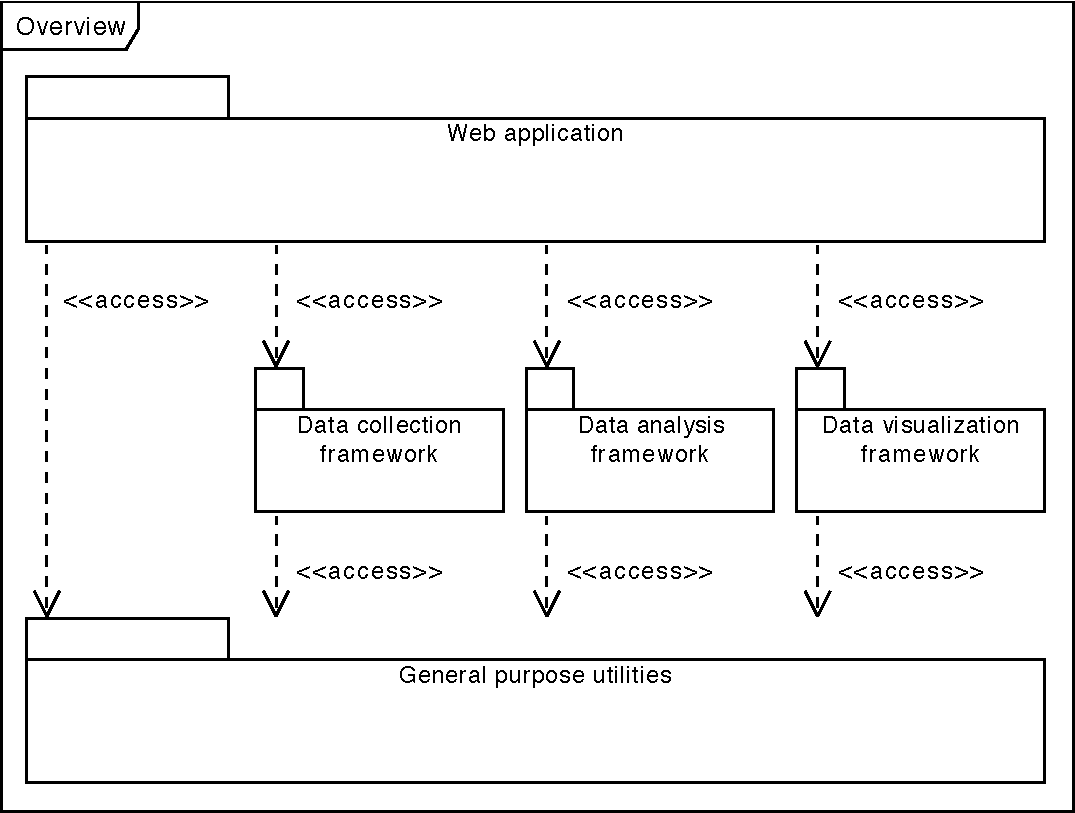
\includegraphics[width=.7\linewidth]{images/simple-overview}
	\caption[Architectural overview of the CSAT software suite.]{Architectural overview resulting from the preliminary analysis presented as a package diagram.}
	\label{fig:simple-overview}
\end{figure}

\p{Pluggable architecture}
As data can come from a plethora of different sources, as the employed visualization techniques may not be adapted to a certain domain, and as the analysis possibilities are endless, it is impossible for the toolkit to cover all possible applications. To obviate to this problem, the design accounts for a completely pluggable architecture, in which new data collectors, visualization engines, and analysis tools can easily be added and removed as the need arises.

\todo{Add a note regarding the content of this chapter we will not speak about implementation specific details related to single components (i.e. the discussion will go down to the interface a module has to implement but stops there). Additional, component-specific, details will be addressed in another chapter. We plan to dedicate a whole chapter to each major component (excluded the common utilities one).}

\section{Data collection framework}

\section{Data analysis framework}

\section{Data visualization framework}

\section{Web application design}

\p{The need for a decoupled wrapper}
One of the main points considered during the design of the toolkit, was the need to fulfill multiple usage scenarios. Each component, e.g., a specific acquisition module, shall be usable both in standalone mode and in concern with other components in an integrated graphical user interface. Usage scenarios for the first case is, for example, the inclusion in a batch processing script or the invocation as a component of a third party library.


\lchapter[tech]{Technology}

\todo{Enumerate and motivate technology related choices.}

\section{State of the art}

\lchapter[collection]{Data collection modules}
\todo{Talk about both the implementation and usage scenarios of each provided collection module.}

\section{Mailing list}

\section{Issue tracker}

\subsection{Mapping tickets to changesets}

\section{Version control repositories}

\subsection{Code dependency discovery}


\lchapter[analysis]{Data analysis modules}
\todo{Talk about both the implementation and usage scenarios of each provided collection module.}


\lchapter[visualization]{Data visualization modules}
\todo{Talk about both the implementation and usage scenarios of each provided collection module.}

\section{Graph visualization engine}

\section{DSM visualization engine}

\lchapter[conclusions]{Conclusions}
